\documentclass{article}
\usepackage{geometry}
\usepackage[T1]{fontenc}
\usepackage[utf8]{inputenc}
\usepackage[pdftex]{graphicx}
\usepackage{multicol}
\usepackage{url}
\usepackage{algorithmic}
\usepackage{algorithm}
\geometry{a4paper}

\title{Global Illumination Rendering using Photon Mapping}
\author{Richard Monette}

\begin{document}
\maketitle
\pagebreak[4]
\tableofcontents
\pagebreak[4]

\section{Acknowledgements}

The following document would not have been possible without the information contained in two key texts: Physically Based Rendering: From Theory to Implementation by Matt Pharr and Greg Humphreys and Realistic Image Synthesis Using Photon Mapping by Henrik Wann Jensen. Many thanks to the authors for creating such wonderful resources.

\pagebreak[4]

\section{Introduction}

This document outlines the theoretical principles, as well as some practical techniques, required in order to implement a physically based global illumination rendering system. First, the rendering equation is presented followed by an explanation of how to solve the components of the rendering equation using distribution ray tracing for direct lighting and photon mapping for the indirect and caustic components. Optimization techniques such as pre-computed irradiances and irradiance caching are then presented. Generally optimization strategies such as low discrepancy sampling, Russian roulette and bounding volume hierarchies are also covered. Finally, the Intaglio rendering system, which implements the previous covered algorithms, is presented along with a collection of experimental results. 

\section{Rendering Fundamentals}

\subsection{The Rendering Equation}

The rendering equation mathematically expresses the transportation of light in models assuming the absence of participating media and as such, can be used to calculate the outgoing radiance at any surface location in a model. Stated in the simplest way:

\begin{equation}
L_{o}(x,\vec{w}) = L_{e}(x,\vec{w}) + L_{r}(x,\vec{w})
\end{equation}

where $L_{o}$ is the outgoing radiance which is the sum of the emitted radiance $L_{e}$ and the reflected radiance $L_{r}$.

\subsection{The Bidirectional Reflectance Distribution Function}

The Bidirectional Reflectance Distribution Function,$f_{r}$, defines the relationship between reflected and incident radiance at a surface point.\cite{nicodemus77}

\begin{equation}
f_{r}(x, \vec{w}', \vec{w}) = \frac{dL_{r}(x,\vec{w})}{dE_{i}(x,\vec{w}')} = \frac{dL_{r}(x,\vec{w})}{L_{i}(x,\vec{w}')(\vec{w}'\cdot\vec{n})d\vec{w}'}
\end{equation}

Thus, given that the BRDF allows for the calculation of the local illumination, we can integrate the incident iradiance over all directions to determine the reflectance in all directions.

\begin{equation}
L_{r}(x, \vec{w}) = \int_\Omega f_{r}(x, \vec{w}', \vec{w})dE(x, \vec{w}') = \int_\Omega f_{r}(x, \vec{w}', \vec{w})L_{i}(x, \vec{w}')(\vec{w}'\cdot\ \vec{n})d\vec{w}
\end{equation}

The BRDF is subjet to the Helmholtz law of reciprocity such that the BRDF is independent of the direction in which the light energy flows:

\begin{equation}
f_{r}(x, \vec{w}', \vec{w}) = f_{r}(x, \vec{w}, \vec{w}')
\end{equation}

It is also important to note that in order for a given BRDF to be said to physically correct it must satistify the condition that it not emit more light than is incident.

\begin{equation}
\int_\Omega f_{r}(x, \vec{w}', \vec{w})L_{i}(x, \vec{w}')(\vec{w}'\cdot\ \vec{n})d\vec{w} \leq 1, \forall \vec{w}
\end{equation}

The reflectance, that is, the fraction of the incident light that is reflected, then can be calculated as follows:

\begin{equation}
p(x) = \frac{\Phi_{r}(x)}{\Phi_{i}(x)} = \frac{\int_{\Omega}\int_{\Omega}f_{r}(x,\vec{w}'\vec{w})L_{i}(x, \vec{w}')(\vec{w}'\cdot\vec{n})d\vec{w}'d\vec{w}}{\int_{\Omega}L_{i}(x, \vec{w}')(\vec{w}'\cdot\vec{w})d\vec{w}'}
\end{equation}

\section{Solving the Rendering Equation}

In order to efficiently evaluate the rendering equation it is beneficial to make the observation that the BRDFs of many material are characterizes by a diffuse element and some specular highlight. Based upon this observation we can re-arrange the BRDF into a split specular/glossy and diffuse terms:

\begin{equation}
f_{r}(x,\vec{w}',\vec{w}) = f_{r,S}(x,\vec{w}',\vec{w}) + f_{r,D}(x,\vec{w}',\vec{w})
\end{equation}

It should be noted that these terms are not by neccessity completely diffuse or specular.
\newline

In a similar manner, the piecewise evaluation of the incoming radiance:

\begin{equation}
L_{i}(x,\vec{w}') = L_{i,l}(x,\vec{w}') + L_{i,c}(x,\vec{w}') + L_{i,d}(x,\vec{w}')
\end{equation}

were $L_{i,l}(x,\vec{w}')$ is the direct illumination from the light sources in the model, $L_{i,c}(x,\vec{w}')$ are the caustics, that light which reached surfaces from the light sources via specular reflection or transmission and $L_{i,d}(x,\vec{w}')$ the indirect illumination, that light which has been diffusely reflected at least one or more times.

\subsection{Direct Lighting} 

In order to render direct lighting using photon mapping, an inordinate amount of photons would be required in order to produce an accurate and noise free image as a result of direct lighting being characterized by high frequency changes in brightness. However, since photon mapping allows for the rendering equation to be solved in a piece-wise manner, it is possible to solve the direct lighting using standard distribution ray tracing.

Likewise, when a ray being cast into the scene intersects a specular surface (reflective or refractive) we trace that ray as in Whitted ray tracing to the next non specular surface. 

Caustics and indirect lighting are then solved using photon mapping.

Solving the direct lighting component of the rendering equation is most efficiently handled by using distribution ray tracing. 

\subsection{Photon Mapping Algorithm}

The photon mapping solution to the rendering equation makes the fundamental observation that it is possible to decouple the lighting information in a given scene from the geometric representation. By exploiting this fact, it is possible to render high quality physically based images in practical time frames. 

Typically, three photon maps are used: the caustics, direct and indirect lighting maps. The nature of caustics being a light focusing phenomena allows for the caustics map to be directly visualized (sometime with some kind of filtering) with an acceptable level of noise.

While the direct illumination can be most practically and efficiently handled using distribution ray tracing, the photon mapping algorithm is better suited to solving the caustic and indirect illumination components of the rendering equation. Typically, a two pass approach is used in the rendering process. First, the requested number of photons are emitted, traced through the scene and finally stored in the appropriate photon map(s). Second, primary visibility and direct lighting is calculated at which time the photon maps are used to add the caustic and indirect illumination contributions. 

\subsubsection{Photon Emission}

Photons are emitted from the light sources in the scene at randomly selected directions in the hemisphere oriented to the normal(s) of the light source. These light sources can be of any type such as point, direct and spotlights as well as physically based lights with arbitrary geometry. In order to generate a photon to be emitted its starting position and direction must be calculated. In the case of a physically based light this can be accomplished by using Monte Carlo sampling to find a surface point on one of the triangles which represent the light sources in the scene. A direction can then be generated in a hemisphere and this direction can be transformed onto the normal of the surface point. When a photon has been generated its path is then traced through the scene and stored in either the direct, indirect or caustic photons maps according to the following rules:

\begin{enumerate}
\item
If a photon first strikes a ‘diffuse’ surface then an entry is added to the direct photon map
\item
If a photon strikes a specular surface (reflective or refractive), it will then store an entry in the caustics map where it next strikes a diffuse surface
\item
Subsequent non-specular bounces are stored in the indirect map
\end{enumerate}

\begin{figure}[h!]
	\centering
	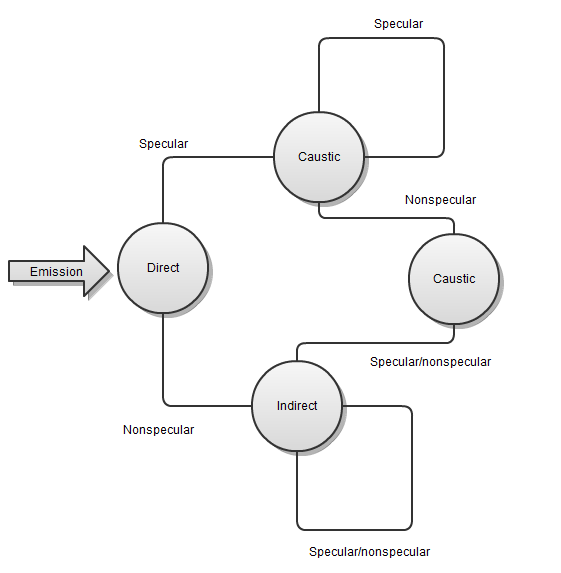
\includegraphics[scale=0.5]{state}
	\caption{State machine indicating where photons are stored based upon surface interactions}
\end{figure}

At each intersection with scene geometry the photon energy is modified by the reflectivity of the surface material at the point of intersection. If the photon still has sufficient energy, it continues along outgoing path which is calculated by using the BRDF of the surface material.

\subsubsection{Photon Storage}

Photons are stored using a kd-tree data structure.\cite{bentley75}\cite{bentleyJuly79}\cite{bentley79} The kd-tree allows for efficient nearest neighbour searching which is required for making radiance estimates in a computationally efficient manner.

\subsubsection{Radiance Estimates}

Once the photon emission, tracing and storage is complete the direct lighting can begin. In order to add the caustic and indirect lighting contributions, estimates can be taken using the photon maps. The reflected radiance is calcuted as:

\begin{equation}
L_{r}(x,\vec{w}) = \int_{\Omega_{x}}f_{r}(x,\vec{w}',\vec{w})L_{i}(x,\vec{w}')(\vec{n}_{x}\cdot\vec{w}')d\vec{w}'
\end{equation}

where $L_{r}$ is the reflected radiance from point $x$ in direction $\vec{w}$ as a result of the incoming radiance $L_{i}$ from hemisphere $\Omega_{x}$ as calculated by $f_{r}$, the BRDF at $x$. A photon map can provide the required information about the incoming flux. Such an estimate can be taken using the following:

\begin{equation}
L_{r}(x,\vec{w}) \approx \frac{1}{\pi r^2}\Sigma_{p=1}^N f_{r}(x,\vec{w}',\vec{w})L_{i}(x,\vec{w}')\triangle\Phi_{p}(x,\vec{w}_{p})
\end{equation}

This formula suggests that a good radiance estimate can be achieved with just enough photons. However, using a sphere based sampling can cause errors where geometry meets at sharp angles. As an example, in corners the sampling sphere on a surface point on the floor would enclose photons which actually reside on the wall area.

\subsubsection{Final Gathering}

A final gathering pass can be performed in order to eliminate the appearance of low frequency noise that is often visible when directly visualizing the indirect photon map. The final gathering consists of sampling the hemisphere over the surface point in order to determine the incident indirect radiance. This sampling can be continued through one or more bounces in order to increase the accuracy. In many situations a single bounce is sufficient to produce adequate results. While hundreds of samples are often required at the first surface point, significantly less are normally required for each subsequent bounce. The extra level of indirection added by using final gathering eliminates low frequency noise that would otherwise be apparent.

\begin{figure}[h!]
	\centering
	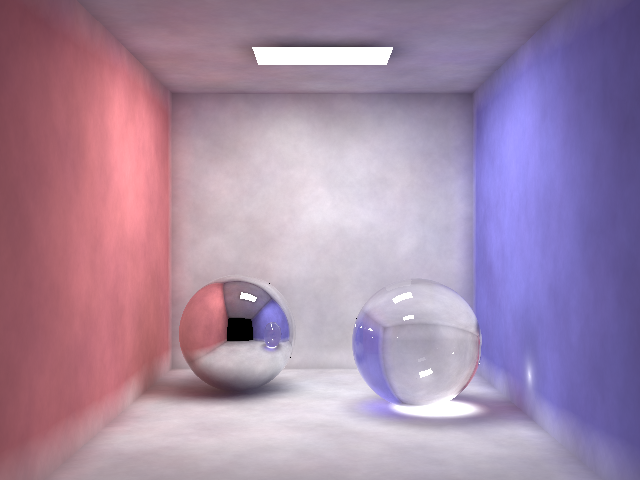
\includegraphics[scale=0.25]{direct}
	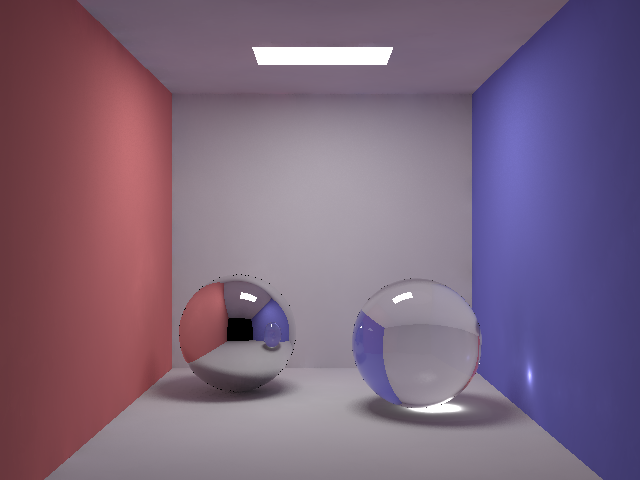
\includegraphics[scale=0.25]{finalgather}
	\caption{Scene rendered using direct visualization of the photon maps and using final gathering}
\end{figure}

\subsection{Practical Photon Mapping Techniques}

\subsubsection{Pre-computed Irradiances}

The final gathering component of rendering is particularly costly as it requires that a significant number of rays not only be cast into the scene and tested for intersection but also that an irradiance estimate must be conducted at each intersection. These irradiance estimates, which typically require 50 - 200 photons are computationally intensive. In order to accelerate this step it is possible to pre-compute irradiance estimates at some subset of the photons in the scene and then directly use those estimates during rendering.\cite{christensen00}

In a practical setting, it is often best to store the pre-computed irradiance values in a separate kd-tree instance which then avoids the need for searching the entire photon map to find an item in the pre-computed irradiance subset. 

\subsubsection{Irradiance Caching}

Another extremely useful optimization approach is to use Irradiance Caching.\cite{ward88} This technique consists of creating irradiance cache entries at points over the scene geometry which can then be interpolated to eliminate the need to perform a full Final Gathering at a given pixel being evaluated. 

\begin{equation}
H = \frac{N}{\Sigma_{1}^N \frac{1}{d_{i}}}
\end{equation}

An irradiance cache entry is characterized by a valid radius which is computed as the harmonic mean of the intersection distances of the Final Gather rays used to compute the cache entry. The harmonic mean is used such that the radius is not overly influenced a few large intersection distances.

\begin{figure}[h!]
	\centering
	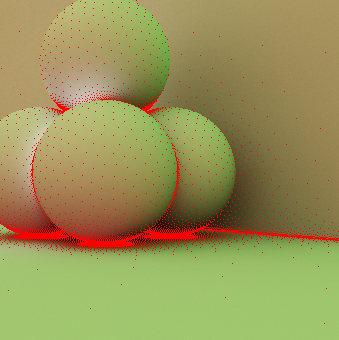
\includegraphics[scale=0.5]{cache}
	\caption{Distribution of irradiance cache points over scene geometry\cite{driscoll}}
\end{figure}

When a surface point is to be shaded the irradiance cache is searched for valid cache entries using the following rules:
\begin{enumerate}
\item
An entry must be withing the valid radius
\item
The entry must have a normal that is sufficiently similar to the point which is being shaded
\item
An entry must not be in front of the point which is being shaded
\end{enumerate}


If no entries are found that match this criteria then a normal final gathering is done and a new entry is added to the cache. However, if one or more valid entries are found, then they are weighted as follows;

\begin{equation}
E = \frac{\Sigma_{1}^N w_{i} E_{i}}{\Sigma_{1}^N w_{i}}
\end{equation}

The irradiance is calculated as the sum of the weights multiplied by individual cache values divided by the sum of the weights. The weight for an entry is defined as;

\begin{equation}
w_{i}=\frac{1}{\vert \vec{P}-\vec{P_{i}} \vert + \sqrt{1 + \vec{N}\cdot\vec{N_{i}}}  }
\end{equation}

When using the irradiance caching algorithm it is usually required that the cache be pre-filled prior to final rendering. This is necessary to avoid the artifacts that are otherwise caused by the adding new values to the cache as rendering progresses.

\section{Efficiency Strategies}

\subsection{Low Discrepancy Sampling}

When using a pure randomly sampling a large number of samples may be required in order to ensure an even distribution within the sample space. However, by using a low discrepancy sampling sequence it is possible to ensure the samples will always be evenly distributed. In practice, this means that it is possible to more effectively sample a space with less samples resulting in less render time. 

\subsubsection{The Hammersely and Halton Sequences}

One usefully low discrepancy sequence is the Hammersely sequence. However, it has the limitation of only being able to be generated when the number of samples required is known. This restriction is not a problem in the example of sampling a light source, as the number of light samples will normally be some constant. In the case of sampling a hemisphere for photon emission this is problematic however, as the number of photons that will need to be emitted in order to achieve the target number of photons stored is unknown. In this case, we can use another low discprepancy sequence known as the Halton sequence which can generate sample values even when the total number required is unknown, although with somewhat more discrepancy than the Hammersely sequence.

\subsection{Russian Roulette}

In order to make the photon tracing step more efficient the Russian Roulette technique can be used.\cite{arvo90} This technique uses probabilistic sampling in order to reduce the amount of calculations while still achieving the correct result. To illustrate the principle, consider tracing a photon through the scene. When the photon intersects some geometry a decision is made using Russian Roulette as to whether it will continue. In the case of our photon we compare its power with a uniformly generated random variable. Since, some amount of the photons will be terminated by this condition, those that continue have their power scaled by the probability of continuation in order to account for the otherwise lost energy.

\subsection{Bounding Volume Hierarchy}

A bounding volume hierarchy is a tree structure in which geometric objects are enclosed by bounding volumes (often axis aligned bounding boxes). These volumes form the leaf nodes of the tree. The leaf nodes are then grouped and bounded by progressively larger volumes, until finally all objects are bounded by one volume. By using a hierarchy potential ray-object intersections can be avoided reducing the intersection comparison time to a logarithmic time operation. This is because child nodes do not need to be tested if a parent fails an intersection test. Furthermore, initial tests are peformed at a corser (and faster) axis aligned bounding box level before per triangle intersection tests are required. Using a bounding volume hierarchy improves performance on all intersection testing reliant components of a rendering solution, such as primary visibility determination as well as photon tracing.

\begin{figure}[h!]
	\centering
	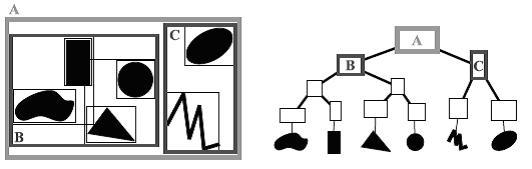
\includegraphics[scale=1.0]{bvh}
	\caption{Bounding volume hierarchy applied to a collection of 2D shapes\cite{wikiBVH}}
\end{figure}

\section{Intaglio Rendering System}

\subsection{Core Features}

The Intaglio rendering system is a 3D rendering application written in C++ that uses the photon mapping algorithm to solve the rendering equation. It has the core primary features:

\begin{enumerate}
\item
Physically based global illumination rendering using photon mapping
\item
Low discrepancy sampling (Halton sequence for photon emission, Hammerseley sequence for direct illumination)
\item
Bounding volume hierarchy ray-triangle intersection structure
\item
Multi-threaded rendering
\end{enumerate}

\subsection{Results}

The following images were produced using the Intaglio rendering system:

\begin{figure}[h!]
	\centering
	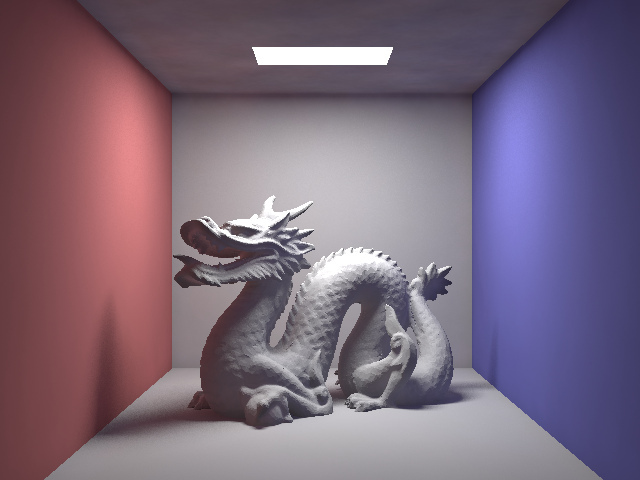
\includegraphics[scale=0.25]{dragon}
	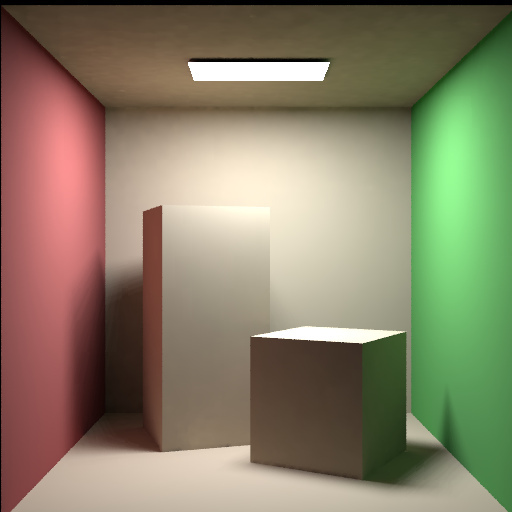
\includegraphics[scale=0.235]{cornell}
	\caption{Dragon model with approximately 100,000 triangles, Cornell box scene}
\end{figure}

\begin{figure}[h!]
	\centering
	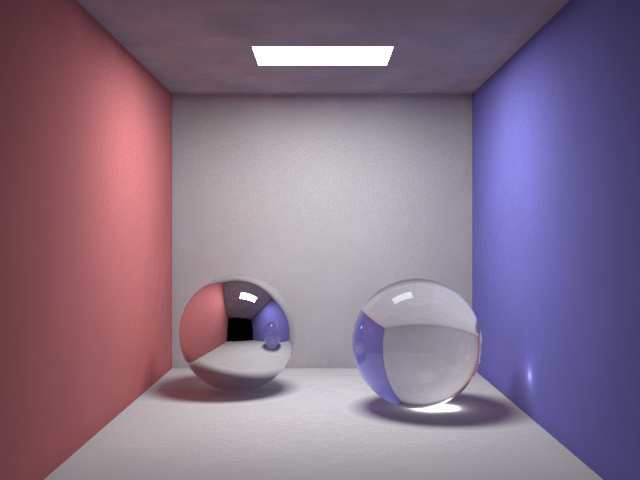
\includegraphics[scale=0.25]{jensen}
	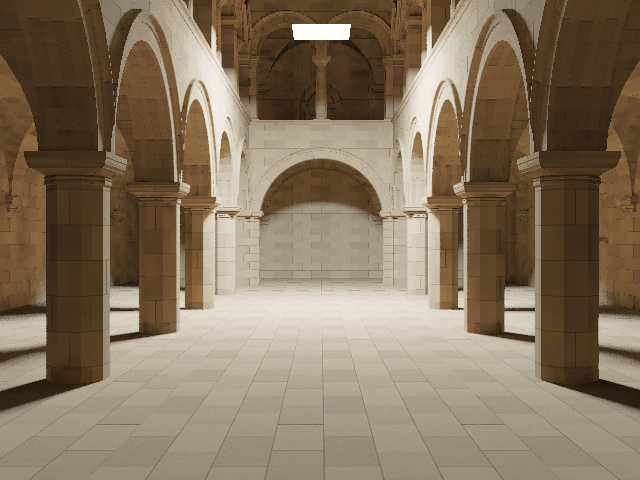
\includegraphics[scale=0.25]{sponza}
	\caption{Jensen box scene, Sponza attrium box scene}
\end{figure}

\begin{figure}[h!]
	\centering
	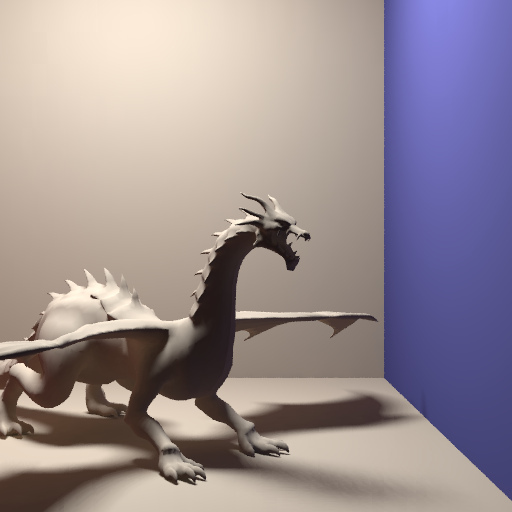
\includegraphics[scale=0.25]{dragon2}
	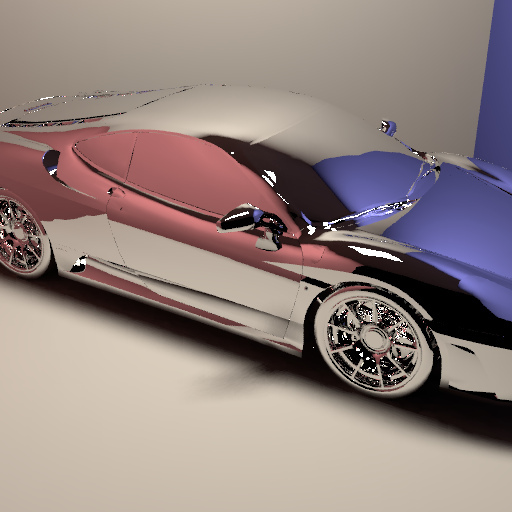
\includegraphics[scale=0.25]{car}
	\caption{Alternate dragon model, Chrome car model}
\end{figure}

\pagebreak[4]
\bibliography{mybib}{}
\bibliographystyle{plain}

\end{document}